\documentclass[tikz,border=1.35mm]{standalone}

\definecolor{fvmadaptedge}{HTML}{8A7E7E}
\usetikzlibrary{arrows.meta}

\definecolor{externalface}{HTML}{8FB9E8}
\definecolor{splitred}{HTML}{AF2525}
\definecolor{centroidgreen}{HTML}{0E8814}

% Face-based isotropic refinement scaffold for an octahedron / square-bipyramid
% diamond cell.
% The eight triangular faces split from face centroids to edge midpoints in red,
% while face centroids connect to the volume centroid in green.
\begin{document}
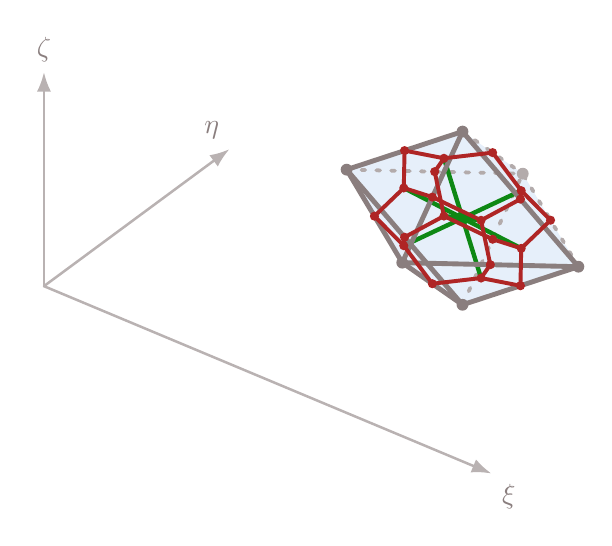
\begin{tikzpicture}[
  x={(20.3mm,-8.5mm)},
  y={(15.3mm,11.3mm)},
  z={(0mm,20mm)},
  line join=round,
  line cap=round,
  outer/.style={draw=fvmadaptedge,line width=0.62mm},
  hidden/.style={draw=fvmadaptedge!65,line width=0.48mm,loosely dotted},
  face/.style={fill=externalface,fill opacity=0.12,draw=none},
  split/.style={draw=splitred,line width=0.50mm},
  centroidedge/.style={draw=centroidgreen,line width=0.56mm},
  axis/.style={draw=fvmadaptedge!60,line width=0.32mm,-{Latex[length=2.5mm,width=1.8mm]}}
]
  % Original vertices.
  \coordinate (L) at (0,0.5,0.55);
  \coordinate (F) at (0.725,0,0.55);
  \coordinate (R) at (1.45,0.5,0.55);
  \coordinate (B) at (0.725,1,0.55);
  \coordinate (T) at (0.725,0.5,1.10);
  \coordinate (S) at (0.725,0.5,0);

  % Edge midpoints.
  \coordinate (mLF) at (0.3625,0.25,0.55);
  \coordinate (mFR) at (1.0875,0.25,0.55);
  \coordinate (mRB) at (1.0875,0.75,0.55);
  \coordinate (mBL) at (0.3625,0.75,0.55);
  \coordinate (mTL) at (0.3625,0.5,0.825);
  \coordinate (mTF) at (0.725,0.25,0.825);
  \coordinate (mTR) at (1.0875,0.5,0.825);
  \coordinate (mTB) at (0.725,0.75,0.825);
  \coordinate (mSL) at (0.3625,0.5,0.275);
  \coordinate (mSF) at (0.725,0.25,0.275);
  \coordinate (mSR) at (1.0875,0.5,0.275);
  \coordinate (mSB) at (0.725,0.75,0.275);

  % Face centroids and volume centroid.
  \coordinate (fTLF) at (0.4833,0.3333,0.7333);
  \coordinate (fTFR) at (0.9667,0.3333,0.7333);
  \coordinate (fTRB) at (0.9667,0.6667,0.7333);
  \coordinate (fTBL) at (0.4833,0.6667,0.7333);
  \coordinate (fSLF) at (0.4833,0.3333,0.3667);
  \coordinate (fSFR) at (0.9667,0.3333,0.3667);
  \coordinate (fSRB) at (0.9667,0.6667,0.3667);
  \coordinate (fSBL) at (0.4833,0.6667,0.3667);
  \coordinate (center) at (0.725,0.5,0.55);

  % Offset computational-coordinate axes.
  \coordinate (Oaxis) at (-1.20,-0.42,-0.18);
  \draw[axis] (Oaxis) -- (1.60,-0.42,-0.18) node[below right,font=\normalsize,text=fvmadaptedge] {$\xi$};
  \draw[axis] (Oaxis) -- (-1.20,1.12,-0.18) node[above left,font=\normalsize,text=fvmadaptedge] {$\eta$};
  \draw[axis] (Oaxis) -- (-1.20,-0.42,1.18) node[above,font=\normalsize,text=fvmadaptedge] {$\zeta$};

  % Faint exterior faces give depth without hiding the split scaffold.
  \path[face] (T) -- (B) -- (L) -- cycle;
  \path[face] (S) -- (B) -- (L) -- cycle;
  \path[face] (T) -- (R) -- (B) -- cycle;
  \path[face] (S) -- (R) -- (B) -- cycle;
  \path[face] (T) -- (L) -- (F) -- cycle;
  \path[face] (S) -- (L) -- (F) -- cycle;
  \path[face] (T) -- (F) -- (R) -- cycle;
  \path[face] (S) -- (F) -- (R) -- cycle;

  % Hidden geometry is drawn before the refinement construction.
  \draw[hidden] (L) -- (B) -- (R);
  \draw[hidden] (T) -- (B);
  \draw[hidden] (S) -- (B);
  \fill[fvmadaptedge!65] (B) circle[radius=0.75mm];

  % Green face-centroid to volume-centroid connections.
  \foreach \p in {fTLF,fTFR,fTRB,fTBL,fSLF,fSFR,fSRB,fSBL} {
    \draw[centroidedge] (center) -- (\p);
  }
  \fill[centroidgreen] (center) circle[radius=0.86mm];

  % Visible exterior wireframe occludes internal centroid connections.
  \draw[outer] (L) -- (F) -- (R);
  \draw[outer] (T) -- (L);
  \draw[outer] (T) -- (F);
  \draw[outer] (T) -- (R);
  \draw[outer] (S) -- (L);
  \draw[outer] (S) -- (F);
  \draw[outer] (S) -- (R);

  % Red face-centroid splits on all eight triangular faces.
  \foreach \p in {mTL,mTF,mLF} {
    \draw[split] (fTLF) -- (\p);
  }
  \foreach \p in {mTF,mTR,mFR} {
    \draw[split] (fTFR) -- (\p);
  }
  \foreach \p in {mTR,mTB,mRB} {
    \draw[split] (fTRB) -- (\p);
  }
  \foreach \p in {mTB,mTL,mBL} {
    \draw[split] (fTBL) -- (\p);
  }
  \foreach \p in {mSL,mSF,mLF} {
    \draw[split] (fSLF) -- (\p);
  }
  \foreach \p in {mSF,mSR,mFR} {
    \draw[split] (fSFR) -- (\p);
  }
  \foreach \p in {mSR,mSB,mRB} {
    \draw[split] (fSRB) -- (\p);
  }
  \foreach \p in {mSB,mSL,mBL} {
    \draw[split] (fSBL) -- (\p);
  }

  % Original vertices are #8a7e7e.
  \foreach \p in {L,F,R,T,S} {
    \fill[fvmadaptedge] (\p) circle[radius=0.75mm];
  }

  % Edge and face refinement nodes are red.
  \foreach \p in {mLF,mFR,mRB,mBL,mTL,mTF,mTR,mTB,mSL,mSF,mSR,mSB,
                  fTLF,fTFR,fTRB,fTBL,fSLF,fSFR,fSRB,fSBL} {
    \fill[splitred] (\p) circle[radius=0.58mm];
  }
\end{tikzpicture}
\end{document}
